\section{Algoritmus SVM}\label{sec:ai-svm}

Metoda podpůrných vektorů (anglicky \emph{support vector machine}, SVM) hledá rozhodovací hranici, která nejen oddělí třídy, ale ponechá mezi nimi co nejširší volný prostor. Nejprve budeme uvažovat lineárně oddělitelná data.

\subsection{Oddělující nadrovina a~maximální okraj}

Pro nový vektor parametrů
\[
    \mathbf{w}=(w_1,\ldots,w_p)\in\R^p
\]
a~\(\theta\in\R\) zavedeme lineární skóre
\[
    g(\mathbf{x})
    =
    \sum_{j=1}^{p}w_jx_j+\theta.
\]
Rozhodovací hranici tvoří nadrovina
\[
    g(\mathbf{x})=0.
\]
V~rovině jde o~přímku, ve třech rozměrech o~rovinu. Klasifikátor přiřadí třídu \(1\) bodům s~\(g(\mathbf{x})\geqslant0\) a~třídu \(0\) bodům s~\(g(\mathbf{x})<0\).

Vzdálenost bodu \(\mathbf{x}\) od této nadroviny je
\[
    \frac{\abs{g(\mathbf{x})}}{\norm{\mathbf{w}}},
    \qquad
    \norm{\mathbf{w}}
    =
    \sqrt{\sum_{j=1}^{p}w_j^2}.
\]
Samotných oddělujících nadrovin může existovat mnoho. SVM volí takovou, jejíž nejbližší body z~obou tříd jsou od hranice co nejdále. Tento nejmenší odstup nazýváme \emph{okraj} (anglicky \emph{margin}).

\begin{figure}[ht]
    \centering
    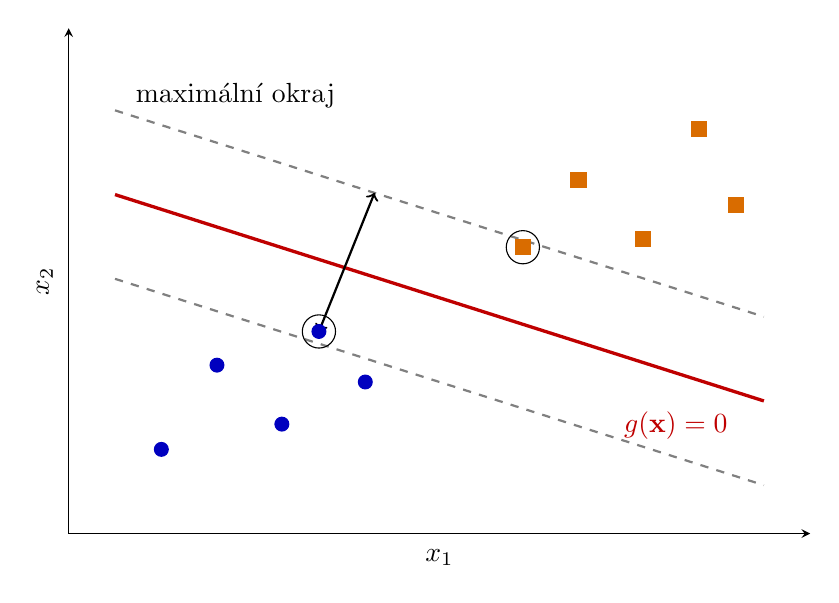
\begin{tikzpicture}
    \begin{axis}[
        width=11cm,height=8cm,
        xmin=0,xmax=8,ymin=0,ymax=6,
        axis lines=left,xlabel={$x_1$},ylabel={$x_2$},
        xtick=\empty,ytick=\empty,
        label style={font=\normalsize},
        every node/.style={font=\normalsize},
        clip=false
    ]
        \addplot[only marks,mark=*,mark size=2.5pt,blue!75!black]
            coordinates{(1,1)(1.6,2)(2.3,1.3)(2.7,2.4)(3.2,1.8)};
        \addplot[only marks,mark=square*,mark size=2.7pt,orange!85!black]
            coordinates{(4.9,3.4)(5.5,4.2)(6.2,3.5)(6.8,4.8)(7.2,3.9)};
        \addplot[red!75!black,very thick,domain=0.5:7.5]{-0.35*x+4.2};
        \addplot[gray,dashed,thick,domain=0.5:7.5]{-0.35*x+3.2};
        \addplot[gray,dashed,thick,domain=0.5:7.5]{-0.35*x+5.2};
        \addplot[only marks,mark=o,mark size=6pt,black]
            coordinates{(2.7,2.4)(4.9,3.4)};
        \node[red!75!black] at (axis cs:6.55,1.28){\(g(\mathbf{x})=0\)};
        \node at (axis cs:1.8,5.2){maximální okraj};
        \draw[<->,thick] (axis cs:2.7,2.4)--(axis cs:3.3,4.045);
    \end{axis}
\end{tikzpicture}

    \caption{Oddělující přímka, maximální okraj a~podpůrné vektory.}
    \label{fig:ai-svm}
\end{figure}

Po vhodném přenásobení \(\mathbf{w}\) a~\(\theta\) můžeme hraniční přímky okraje zapsat
\[
    g(\mathbf{x})=1
    \qquad\text{a}\qquad
    g(\mathbf{x})=-1.
\]
Jejich vzájemná vzdálenost je
\[
    \frac{2}{\norm{\mathbf{w}}}.
\]
Body ležící na hranicích okraje nazýváme \emph{podpůrné vektory}. Právě ony polohu optimální hranice přímo určují. Posun bodu ležícího daleko od okraje ji obvykle nezmění, zatímco posun podpůrného vektoru ano.

Šířku okraje nemůžeme zvětšovat libovolným přenásobením parametrů, protože současně požadujeme, aby trénovací objekty ležely na správné straně hraničních nadrovin. Označíme-li třídy hodnotami \(\tilde y_i=2y_i-1\in\set{-1,1}\), tvrdý okraj splňuje podmínky
\[
    \tilde y_i g(\mathbf{x}_i)\geqslant1
    \qquad\text{pro všechna }i.
\]
Maximalizace šířky \(2/\norm{\mathbf{w}}\) je za těchto podmínek ekvivalentní minimalizaci \(\frac12\norm{\mathbf{w}}^2\).

\subsection{Neoddělitelná data a~měkký okraj}

Reálná data často nelze bez chyby oddělit jedinou nadrovinou. SVM proto může použít \emph{měkký okraj}: připustí některé body uvnitř okraje nebo dokonce na chybné straně hranice. Nastavení modelu pak představuje kompromis mezi dvěma cíli:
\begin{itemize}
    \item mít okraj co nejširší;
    \item mít co nejméně závažných porušení a~chybných klasifikací.
\end{itemize}
Parametr \(C>0\) určuje cenu porušení. Velké \(C\) chyby silně trestá a~obvykle vede k~užšímu okraji. Menší \(C\) dovolí více porušení, ale může vytvořit stabilnější širší hranici. Hodnotu \(C\) volíme pomocí validačních dat.

Míru porušení pro objekt \(i\) lze vyjádřit \emph{pantovou ztrátou} (anglicky \emph{hinge loss})
\[
    \ell_i
    =
    \max\set{0,1-\tilde y_i g(\mathbf{x}_i)}.
\]
Je-li objekt správně za okrajem, platí \(\ell_i=0\). Bod uvnitř okraje má kladnou ztrátu, a~bod na chybné straně rozhodovací hranice ztrátu větší než \(1\). Trénování měkkého okraje lze proto zapsat jako minimalizaci
\[
    \frac12\norm{\mathbf{w}}^2
    +
    C\sum_{i=1}^{n}\ell_i.
\]

Lineární hranice nemusí stačit ani po povolení chyb. Jednou možností je převést objekty do prostoru s~dalšími znaky, v~němž je lze oddělit nadrovinou. Jádrový trik (anglicky \emph{kernel trick}) umožňuje některé takové výpočty provést bez explicitního vytváření všech nových souřadnic. Výsledná hranice v~původním prostoru pak může být nelineární.

Jádro musí vhodným způsobem vyjadřovat podobnost dvojice objektů. Volba lineárního jádra ponechá původní nadrovinu, polynomiální nebo gaussovské jádro umožní zakřivené hranice. Složitější hranice však nemusí lépe zobecňovat, a~proto typ jádra i~jeho parametry volíme podle validačních dat.

\subsection{Vlastnosti a~použití}

Mezi výhody SVM patří jasná geometrická interpretace, možnost nelineárních hranic a~skutečnost, že hranici přímo určuje jen část trénovacích objektů. Metoda může dobře fungovat i~při větším počtu znaků.

Nevýhodou je citlivost na měřítko dat a~na volbu \(C\) a~jádra. U~velkých datových souborů může být trénování náročné a~výstup modelu nemá bez další úpravy přímou pravděpodobnostní interpretaci jako výstup logistické regrese. Typicky se SVM používá pro klasifikaci textu, obrazových znaků nebo biologických dat, zejména není-li počet trénovacích objektů extrémně velký.

Podpůrné vektory zároveň poskytují užitečnou kontrolu modelu. Pokud se jejich malá změna výrazně projeví na rozhodovací hranici, může být model citlivý na šum nebo odlehlá pozorování. Velký počet podpůrných vektorů zase naznačuje, že třídy nejsou zvolenými znaky dobře oddělené.

\warningbox{Stejně jako u~\(k\)-NN je před trénováním SVM obvykle nutné standardizovat nebo normalizovat vstupní znaky. Jinak geometrický okraj odráží především rozdílné jednotky a~měřítko.}

\begin{remark}
    Základy metody podpůrných vektorů vznikaly v~pracích Vladimira Vapnika a~Alexeje Červoněnkise už v~60.~letech 20.~století. Dnes běžnou variantu s~měkkým okrajem popsali Corinna Cortesová a~Vladimir Vapnik roku 1995.
\end{remark}

\subsection{Pseudokód a~implementace}

Pro názornou implementaci použijeme lineární SVM a~stochastický podgradientní sestup. Místo parametru \(C\) budeme regulaci zapisovat pomocí nového parametru \(\lambda>0\) v~ekvivalentně škálovaném cíli
\[
    \frac{\lambda}{2}\norm{\mathbf{w}}^2
    +
    \frac1n\sum_{i=1}^{n}
    \max\set{0,1-\tilde y_i g(\mathbf{x}_i)}.
\]
Větší \(\lambda\) silněji zmenšuje váhy a~upřednostňuje širší okraj; jeho role je tedy opačná než role \(C\).

V~každém kroku nejprve váhy mírně zmenšíme kvůli členu \(\frac{\lambda}{2}\norm{\mathbf{w}}^2\). Pokud vybraný objekt porušuje okraj, přidáme navíc opravu ve směru \(\tilde y_i\mathbf{x}_i\) a~upravíme práh. Jde o~zjednodušený výukový postup; plnohodnotné knihovny používají rychlejší optimalizační metody a~pečlivější volbu rychlosti učení.

\begin{algorithm}
    \caption{\textsc{svm-sgd}}
    \label{alg:ai-svm}
    \KwIn{Trénovací množina \(D\), rychlost učení \(\eta>0\), regulace \(\lambda>0\) a~počet epoch \(T\)}
    \(\mathbf{w}\gets\mathbf{0}\), \(\theta\gets0\)\\
    \For{\(e\gets1,2,\ldots,T\)}{
        \ForEach{\textup{objekt \((\mathbf{x}_i,y_i)\in D\)}}{
            \(\tilde y_i\gets2y_i-1\)\\
            \(\mathbf{w}\gets(1-\eta\lambda)\mathbf{w}\)\\
            \If{\(\tilde y_i(\sum_{j=1}^{p}w_jx_{ij}+\theta)<1\)}{
                \(\mathbf{w}\gets\mathbf{w}+\eta\tilde y_i\mathbf{x}_i\)\\
                \(\theta\gets\theta+\eta\tilde y_i\)
            }
        }
    }
    \KwOut{Klasifikátor \(h(\mathbf{x})=1\), pokud \(\sum_{j=1}^{p}w_jx_j+\theta\geqslant0\), jinak \(0\)}
\end{algorithm}

Program~\ref{lst:ai-svm} odpovídá tomuto pseudokódu. Metoda \texttt{decision\_function} vrací podepsané skóre: jeho znaménko určuje třídu a~jeho absolutní hodnota vyjadřuje vzdálenost od hranice pouze po vydělení normou vah. Metoda \texttt{predict} proto ke klasifikaci používá jen znaménko.

\lstinputlisting[
    caption={Lineární SVM trénované stochastickým podgradientním sestupem.},
    label={lst:ai-svm}
]{07-ai/code/svm.py}

Příklad obsahuje dvě lineárně oddělitelné skupiny bodů. Po natrénování program vypíše parametry hranice a~třídy několika nových objektů. Před použitím na reálných datech bychom vstupní znaky standardizovali a~hodnoty \(\lambda\), \(\eta\) i~počet epoch zvolili podle validační množiny.
